\chapter{saMKAyxvinAyxsa}

oMdu hU toVTadalilx elegaLanunx noVDidAga avugaLalilxruva vinAyxsavanunx noVDi AshacxyaRvAgutatxde! maneya muMde iTiTxruva raMgoVliyanunx noVDidAga reVKegaLa vinAyxsa acacxrigoLisutatxde. parxtiyobabx manuSayxnalUlx avana vayxkitxtavxkekx saMbaMdhisida oMdu visheVSa guNaviruvaMte parxtiyoMdu saMKeyxyalUlx oMdu visheVSa guNavirutatxde. kelavu saMKeyxgaLalalxMtU vinAyxsa balu AshacxyaRkaravAda guNagaLirutatxve. 

udAharaNege : $12345654321$ idoMdu mAlAsaMKeyx. heVgeV OdidarU eDagaDeyiMda, balagaDeyiMda oMdeV!

I samaBinanxrAshigaLanunx noVDi AnaMda paDabahudu.
$$
\frac{2}{3} = \frac{3}{6} = \frac{79}{158}
$$

idaralilx $1$ riMda $9$ ravaregina elAlx saMKeyxgaLU oMdoMdeV bAri baMdive. I vayxvakalanadalilx $1, 4, 6$ matutx $7$ eMba aMkagaLeV punarAvatiRsiruvudanunx noVDi!
$$
7641-1467 = 6174
$$

I saMKAyxvinAyxsa balu sogasAgiyAgide!

\eject

$42857$ I saMKeyxya muMdakekx $1$ nunx seVrisidare, baruva saMKeyxyu hiMdakekx $1$ nunx seVrisidare baruva saMKeyxyu $3$ raSATxgutatxde.
$$
142857 \times 3 = 428571
$$

AhA! I saMKeyxgaLa opapxMdaveV namagoMdu AnaMdada anuBava
\begin{align*}
0, ~ 999, ~999 \div 9 & =111, ~111\\
1, ~999,~998 \div 9& =222, ~222\\
2,~999,~997 \div 9 &=333, ~ 333\\
3,~999, ~996 \div 9&=444, ~444
\end{align*}

abAbx! Enu AshacxyaR $1^3 + 5^3 + 3^3 = 153$

AhA! Enu sogasu $123456789 \times 90=10101010$

I guNAkArada visheVSa gamanisi
$$
3 \times 4 = 12
$$
ililx $1$ riMda $4$ra tanaka iruva elalx aMkigaLU oMdoMdu sala baMdive ideV riVti $13 \times 4 = 52$

ililx $1$ riMda $5$ra tanaka iruva elalx aMkigaLU oMdoMdu sala baMdive mAnavaru sahasArxru vaSaRgaLiMda aMkegaLoDane ATavADidAdxre. aneVka rahasayxvanunx kaMDukoMDidAdxre. vinoVdakaravAda ATagaLanunx kalipxsidAdxre. hosa hosa namUneya vUyxhagaLanunx yaMtarxgarxMthagaLalilx barediTiTxdAdxre. I rahasayxgaLalilx camatAkxravirabahudu.  Adare shAsitxrXVyavAda viSayavU aDagiruvuduMTu. oMdoMdu veVLe hiVge mADidare, hAgeVkAgutatxde? matotxMdu riVti mADidare EnAgutatxde? eMdu avareV yoVcisirabahudu.

$1729$ eMba saMKeyxyu eraDu riVtiyalilx eraDu GanasaMKeyxgaLa motatxvAgiruva kaniSaThx saMKeyxyAgide.
$$
12^3 + 1^3 =10^3 + 9 ^3 = 1729
$$
%\begin{wrapfigure}{o}{0.4\textwidth}
 % \centering\includegraphics[scale=0.8]{src/figures/Ramanujan.eps}
   % \end{wrapfigure}
\begin{figure}[H]
\centering\includegraphics[scale=0.8]{src/figures/Ramanujan.eps}

{\bf citarx~: ~shirxVnivAsa rAmAnujanf}
\end{figure}
idu Adhunika BAratiVya gaNitajacnx~ shirxVnivAsa rAmAnujanfna saMKeyx mAyA cwkada bagegx vividha riVtiyide.

AlfPerxVDf  masanxrf na mAyA cwka noVDi!

ADaDxsAlu matutx kaMba sAlugaLu guNisidAga guNalabadhx $120$ barutatxde Adare kaNaRgaLa guNalabadhxdiMda $120$ baruvudilalx
\begin{center}
\begin{tabular}{|c|c|c|}
\hline
$10$ & $12$ & $1$\\
\hline
$4$ & $5$ & $15$\\
\hline
$3$ & $5$ & $8$\\
\hline
\end{tabular}
\end{center}

I karxmAgata eraDu saMKeyxgaLa motatxda vagaRmUla, oMdu aviBAjayx saMKeyxyAgiruvudanunx noVDi!
\begin{align*}
  \sqrt{(4+5)} & = 3\\
  \sqrt{(12+13)} & = 5\\
  \sqrt{(24+25)} &= 7
\end{align*}
(Adare elAlx karxmAgata saMKeyxgaLigU I sUtarx anavxyisuvudilalx)

oTiTxnalilx saMKeyxgaLalilx vinAyxsa, AnaMda, AshacxyaR kutUhalavAgide! 



